\documentclass[11pt, oneside, a4paper]{article}

\usepackage{courier}

\usepackage{enumitem}

\usepackage{amssymb}
\usepackage{amsmath}

\usepackage{textcomp}

\usepackage[
	includehead,
	includefoot,
	headheight=30pt,
	left=0.79in,
	right=0.79in,
	top=0.39in,
	bottom=0in,
	headsep=10pt
]{geometry}

\usepackage{fancyhdr}
\usepackage{graphicx}
\usepackage{verbatim}
\usepackage{parskip}

\usepackage{tabu}

\usepackage[utf8]{inputenc}
\usepackage[T1]{fontenc}
\usepackage[croatian]{babel}

\newcommand{\contestname}{HONI 2014/2015}
\newcommand{\contesttime}{5. kolo, 17. siječnja 2015.}
\newcommand{\taskname}{}
\newcommand{\timelimit}{}
\newcommand{\memorylimit}{}
\newcommand{\score}{}

\lhead{%
	\fontfamily{\sfdefault}
	\fontsize{10pt}{1.1em}
	\bfseries
	\selectfont
	\contestname\\%
	\contesttime%
}	

\rhead{%
	\fontfamily{\sfdefault}
	\fontsize{10pt}{1.1em}
	\bfseries
	\selectfont
	Zadatak \taskname\\%
	\timelimit, \memorylimit, \score%
}

\cfoot{}

\renewcommand{\headrule}{
\kern 1pt
\hrule width \hsize
\kern 1pt
\hrule width \hsize
}

\newcommand{\naslov}[1]{
\begin{center}
\fontfamily{\sfdefault}
\fontsize{10pt}{1.1em}
\bfseries
\selectfont
\uppercase{#1}
\end{center}
}

\setlength{\parindent}{0pt}

\pagestyle{fancy}

\begin{document}

\pagebreak
\renewcommand{\taskname}{STRAVA}
\renewcommand{\timelimit}{1 sekunda}
\renewcommand{\memorylimit}{32 MB}
\renewcommand{\score}{20 bodova}

Duž Ulice brijestova \textbf{s obje strane} posađeni su, pogađate, brijestovi. Svaka dva susjedna brijesta međusobno su razmaknuta $K$ metara te je poznato da se na početku i kraju ulice nalazi po jedan brijest. Nakon nemilih događaja, stanovnici ulice odlučili su svaki treći brijest zamijeniti hrastom. 

Ako znate da je ulica dugačka $L$ metara, odredite koliko je brijestova, a koliko hrastova posađeno u Ulici brijestova. 

\strut

\naslov{ulazni podaci}

U jedinom redu ulaza nalaze se brojevi $K$ i $L$ ($1 \leqslant K < L \leqslant 1000$, $L$ je djeljiv s $K$) iz teksta zadatka.

\strut

\naslov{izlazni podaci}

Ispišite dva cijela broja odvojena razmakom koji redom predstavljaju broj brijestova i broj hrastova koji se nalaze u Ulici brijestova.

\textbf{Napomena:} brojevi $K$ i $L$ bit će takvi da se u ulici nalaze barem 3 stabla.

\strut

\naslov{primjeri test podataka}

\begin{center}
\fontfamily{\ttdefault}
\fontsize{10pt}{1em}
\selectfont
\begin{tabu}to 0.99\textwidth{|X[1]|X[1]|X[1]|}
\hline
& & \\ 
\rowfont{\fontsize{10pt}{1em}\bfseries}
ulaz & ulaz & ulaz\\
\verbatiminput{strava/strava.dummy.in.1} &
\verbatiminput{strava/strava.dummy.in.2} & 
\verbatiminput{strava/strava.dummy.in.3} \\
\rowfont{\fontsize{10pt}{1em}\bfseries}
izlaz & izlaz & izlaz\\
\verbatiminput{strava/strava.dummy.out.1} &
\verbatiminput{strava/strava.dummy.out.2} & 
\verbatiminput{strava/strava.dummy.out.3} \\
\hline
\end{tabu}
\end{center}

{
\fontsize{10pt}{1em}
\selectfont
%\textbf{Pojašnjenje prvog primjera:} pojašnjenje pojašnjenje pojašnjenje \\
%\textbf{Pojašnjenje drugog primjera:} pojašnjenje pojašnjenje pojašnjenje
}

\pagebreak
\renewcommand{\taskname}{UŽAS}
\renewcommand{\timelimit}{1 sekunda}
\renewcommand{\memorylimit}{32 MB}
\renewcommand{\score}{30 bodova}

Živite u Ulici brijestova na kućnom broju $X$ i želite doći do svojega prijatelja koji živi na kućnom broju $Y$ na istroj strani ulice. Na putu nećete nikada prelaziti cestu, jer ste već na pravoj strani.

Opće je poznato da su kuće čiji su kućni brojevi djeljivi s 4 uklete. Izračunajte kraj koliko ukletih kuća ćete proći na putu od svoje kuće do prijatelja (računajući i vašu i prijateljevu kuću ako su uklete). 

\textbf{Napomena:} s jedne strane ulice nalaze se parni kućni brojevi, a s druge strane neparni.

\strut

\naslov{ulazni podaci}

U jedinom retku ulaza nalaze se dva različita prirodna broja $X$ i $Y$ ($1 \leqslant X, Y \leqslant 1\,000$), vaš i prijateljev kućni broj.

\naslov{izlazni podaci}

U prvi i jedini redak izlaza ispišite jedan cijeli broj, broj ukletih kuća kraj kojih ćete proći na putu.

\strut

\naslov{primjeri test podataka}

\begin{center}
\fontfamily{\ttdefault}
\fontsize{10pt}{1em}
\selectfont
\begin{tabu}to 0.99\textwidth{|X[1]|X[1]|}
\hline
& \\ 
\rowfont{\fontsize{10pt}{1em}\bfseries}
ulaz & ulaz \\
\verbatiminput{uzas/uzas.dummy.in.1} & 
\verbatiminput{uzas/uzas.dummy.in.2} \\
\rowfont{\fontsize{10pt}{1em}\bfseries}
izlaz & izlaz \\
\verbatiminput{uzas/uzas.dummy.out.1} & 
\verbatiminput{uzas/uzas.dummy.out.2} \\
\hline
\end{tabu}
\end{center}

{
\fontsize{10pt}{1em}
\selectfont
\textbf{Pojašnjenje prvog primjera:} Proći ćete kraj ukletih kuća sa kućnim brojevima 4, 6 i 8. \\
%\textbf{Pojašnjenje drugog primjera:} pojašnjenje pojašnjenje pojašnjenje
}

\pagebreak
\renewcommand{\taskname}{FUNGHI}
\renewcommand{\timelimit}{1 sekunda}
\renewcommand{\memorylimit}{32 MB}
\renewcommand{\score}{50 bodova}

Nakon što su pojeli sve kolačiće s vještičine kuće, Ivica i Marica naručili su jumbo pizzu. Pizza je uskoro stigla, narezana na osam komada. Ivica i Marica pizzu će podijeliti popola tako da svatko od njih dobije jedan cijeli "polukrug" pizze, tj. četiri uzastopna komada.

Marica jako voli šampinjone i želi ih dobiti što više. Budući da se na nekim komadima pizze nalazi manje, a na nekima više šampinjona, Marica je zamolila Ivicu da pizzu podijele tako da se na njezinim komadima nađe što više šampinjona.

Pomozite Ivici i Marici! Oni će vam reći koliko se šampinjona nalazi na svakom od osam komada pizze, a vi pronađite \textbf{najveći ukupan broj šampinjona koji Marica može dobiti}. Sljedeća slika prikazuje najbolju podjelu za drugi test primjer niže (brojem 1. označen je prvi komad naveden u ulaznim podacima):

\begin{center}
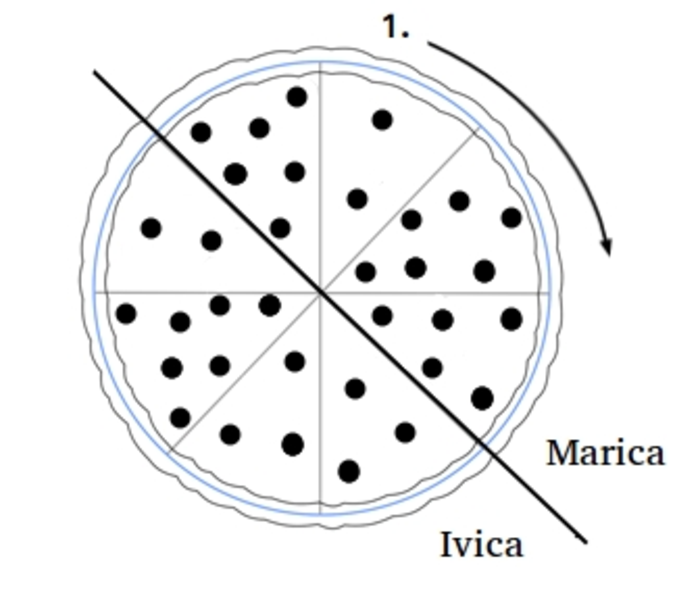
\includegraphics[width=.4\linewidth]{funghi/slika.pdf}
\end{center}

\strut

\naslov{ulazni podaci}

U osam redaka nalazi se po jedan cijeli broj $\check{S}_i$ ($0 \leqslant \check{S}_i \leqslant 50$, $i = 1, 2, \ldots, 8$).
Ovi su brojevi količine šampinjona na komadima pizze, pri čemu su komadi dani redom u smjeru kazaljke na satu.

\strut

\naslov{izlazni podaci}

U jedini redak ispišite traženi broj iz teksta zadatka.

\strut

\naslov{primjeri test podataka}

\begin{center}
\fontfamily{\ttdefault}
\fontsize{10pt}{1em}
\selectfont
\begin{tabu}to 0.99\textwidth{|X[1]|X[1]|}
\hline
& \\ 
\rowfont{\fontsize{10pt}{1em}\bfseries}
ulaz & ulaz \\
\verbatiminput{funghi/funghi.dummy.in.1} & 
\verbatiminput{funghi/funghi.dummy.in.2} \\
\rowfont{\fontsize{10pt}{1em}\bfseries}
izlaz & izlaz \\
\verbatiminput{funghi/funghi.dummy.out.1} & 
\verbatiminput{funghi/funghi.dummy.out.2} \\
\hline
\end{tabu}
\end{center}

{
\fontsize{10pt}{1em}
\selectfont
%\textbf{Pojašnjenje prvog primjera:} pojašnjenje pojašnjenje pojašnjenje \\
%\textbf{Pojašnjenje drugog primjera:} pojašnjenje pojašnjenje pojašnjenje
}

\pagebreak
\renewcommand{\taskname}{ZMIJA}
\renewcommand{\timelimit}{1 sekunda}
\renewcommand{\memorylimit}{32 MB}
\renewcommand{\score}{80 bodova}

Mirko radi kopiju popularne računalne igre "Zmijica". U igri kontrolirate zmijičine kretnje po ekranu dimenzija $R \cdot S$ piksela, a cilj igre je pokupiti sve jabučice koje se nalaze na ekranu. 

Nažalost, Mirkova implementacija nije baš bajna pa se tijek igre razlikuje od originala. Slijedi opis Mirkove igre:
\begin{itemize}
\item za razliku od originala, jabučice se ne pojavljuju nasumično na ekranu, već su na početku igre poznate pozicije svih jabuka
\item na početku igre, zmijica se nalazi u donjem lijevom kutu ekrana i gleda udesno
\item postoje dvije tipke u igri, označene s A i B
\item pritiskom na tipku A, zmijica se pomiče za jedan piksel u smjeru u kojem trenutno gleda. Ako bi zmijica tim pomakom izašla iz ekrana, onda se ne događa ništa.
\item pritiskom na tipku B, zmijica se pomiče za jedan piksel prema gore i mijenja smjer gledanja za 180\textdegree
\item kada se zmijica pomakne na piksel na kojem se nalazi jabuka, pojede ju, ali ne naraste kao u originalu
\end{itemize}

Vaš zadatak je sljedeći: za zadane pozicije jabučica na početku igre odredite \textbf{najmanji broj pritisaka tipki} potreban da zmijica skupi \textbf{sve jabučice}.

\strut

\naslov{ulazni podaci}

U prvom retku nalaze se prirodni brojevi $R$ i $S$ ($2 \leqslant R, S \leqslant 1\,000$), visina i širina ekrana.

U svakom od idućih $R$ redaka nalazi se točno $S$ znakova. Ti znakovi predstavljaju sadržaj ekrana. Na pikselima gdje su jabučice bit će znak 'J', na praznim pikselima znak '.'.

U donjem lijevom kutu nalazit će se znak 'Z' koji predstavlja zmijicu na njenoj početnoj poziciji.

\strut

\naslov{izlazni podaci}

U jedini redak izlaza ispišite traženi najmanji broj pritisaka tipki.

\strut

\naslov{primjeri test podataka}

\begin{center}
\fontfamily{\ttdefault}
\fontsize{10pt}{1em}
\selectfont
\begin{tabu}to 0.99\textwidth{|X[1]|X[1]|X[1]|}
\hline
& & \\ 
\rowfont{\fontsize{10pt}{1em}\bfseries}
ulaz & ulaz & ulaz\\
\verbatiminput{zmija/zmija.dummy.in.1} &
\verbatiminput{zmija/zmija.dummy.in.2} & 
\verbatiminput{zmija/zmija.dummy.in.3} \\
\rowfont{\fontsize{10pt}{1em}\bfseries}
izlaz & izlaz & izlaz\\
\verbatiminput{zmija/zmija.dummy.out.1} &
\verbatiminput{zmija/zmija.dummy.out.2} & 
\verbatiminput{zmija/zmija.dummy.out.3} \\
\hline
\end{tabu}
\end{center}

{
\fontsize{10pt}{1em}
\selectfont
\textbf{Pojašnjenje prvog primjera:} Najkraći niz pritisaka tipki potreban da zmijica skupi sve jabučice je BBAAABB. \\
%\textbf{Pojašnjenje drugog primjera:} pojašnjenje pojašnjenje pojašnjenje
}

\pagebreak
\renewcommand{\taskname}{TRAKTOR}
\renewcommand{\timelimit}{2 sekunde}
\renewcommand{\memorylimit}{32 MB}
\renewcommand{\score}{100 bodova}

Mirko je za Božić dobio novi super traktor kojim može brati gljive! Gljive rastu na livadi kvadratnog oblika koju možemo smjestiti u koordinatnu ravninu tako da joj je donji lijevi rub u točki $(1, 1)$ a gornji desni u točki $(10^5, 10^5)$.

U početnom trenutku na livadi nema gljiva, no narast će ih ukupno $N$ i to tako da svake sekunde naraste točno jedna nova na nekom praznom mjestu na livadi. 

Štedljivi Mirko želi \emph{samo jednom} vožnjom traktora ubrati barem $K$ gljiva. Svoj put započinje u jednoj od točaka livade i može voziti samo paralelno njenim stranicama ili dijagonalama. 
Mirkov traktor je super brz, \textbf{proizvoljno veliku udaljenost prelazi u zanemarivom vremenu}. Zbog silne brzine, Mirko \emph{ne može skretati} za vrijeme vožnje.

Pomozite Mirku i odredite \textbf{najmanji broj sekundi} nakon kojih može ubrati željeni broj gljiva. 

\strut

\naslov{ulazni podaci}

U prvom retku nalaze se prirodni brojevi $N$ ($2 \leqslant N \leqslant 10^6$) i $K$ ($2 \leqslant K \leqslant N$), broj gljiva koje će izrasti i broj gljiva koji Mirko želi ubrati.

U sljedećih $N$ redaka nalaze se po dva prirodna broja $X_i$ i $Y_i$ ($1 \leqslant X_i, Y_i \leqslant 10^5$), koordinate $i$-te gljive koja je narasla na livadi.

\naslov{izlazni podaci}

U jedini redak ispišite traženi najmanji broj sekundi.
Ako Mirko ne može ubrati $K$ gljiva jednom vožnjom, ispišite -1.

\naslov{bodovanje}

U test podacima vrijednima ukupno 50\% bodova vrijedit će $1 \leqslant X_i, Y_i \leqslant 300$.

\strut

\naslov{primjeri test podataka}

\begin{center}
\fontfamily{\ttdefault}
\fontsize{10pt}{1em}
\selectfont
\begin{tabu}to 0.99\textwidth{|X[1]|X[1]|X[1]|}
\hline
& & \\ 
\rowfont{\fontsize{10pt}{1em}\bfseries}
ulaz & ulaz & ulaz\\
\verbatiminput{traktor/traktor.dummy.in.1} &
\verbatiminput{traktor/traktor.dummy.in.2} & 
\verbatiminput{traktor/traktor.dummy.in.3} \\
\rowfont{\fontsize{10pt}{1em}\bfseries}
izlaz & izlaz & izlaz\\
\verbatiminput{traktor/traktor.dummy.out.1} &
\verbatiminput{traktor/traktor.dummy.out.2} & 
\verbatiminput{traktor/traktor.dummy.out.3} \\
\hline
\end{tabu}
\end{center}

{
\fontsize{10pt}{1em}
\selectfont
\textbf{Pojašnjenje prvog primjera:} Mirko svoju vožnju započinje u točki $(1, 2)$ i kreće se prema gljivi s koordinatama $(4, 5)$. \\
%\textbf{Pojašnjenje drugog primjera:} pojašnjenje pojašnjenje pojašnjenje
}

\pagebreak
\renewcommand{\taskname}{ZGODAN}
\renewcommand{\timelimit}{1 sekunda}
\renewcommand{\memorylimit}{32 MB}
\renewcommand{\score}{120 bodova}

Prirodan broj nazivamo zgodnim ako su mu svake dvije susjedne znamenke različite parnosti.
Za dani prirodan broj $N$, koji je njemu najbliži zgodni broj?

\textbf{Napomene:} Jednoznamenkasti brojevi su zgodni. Udaljenost dvaju brojeva apsolutna je vrijednost njihove razlike.

\strut

\naslov{ulazni podaci}

U jedinome retku nalazi se prirodan broj $N$ koji ima najviše tisuću znamenaka i nije zgodan.

\strut
\naslov{izlazni podaci}

U jedini redak ispišite traženi najbliži zgodni broj. Ako postoje dva najbliža broja, ispišite oba, odvojene razmakom.

\strut
\naslov{bodovanje}

U test podacima ukupno vrijednima 56 bodova vrijedit će $N < 10^9$.

\strut

\naslov{primjeri test podataka}

\begin{center}
\fontfamily{\ttdefault}
\fontsize{10pt}{1em}
\selectfont
\begin{tabu}to 0.99\textwidth{|X[1]|X[1]|}
\hline
& \\ 
\rowfont{\fontsize{10pt}{1em}\bfseries}
ulaz & ulaz \\
\verbatiminput{zgodan/zgodan.dummy.in.1} &
\verbatiminput{zgodan/zgodan.dummy.in.2} \\
\rowfont{\fontsize{10pt}{1em}\bfseries}
izlaz & izlaz \\
\verbatiminput{zgodan/zgodan.dummy.out.1} &
\verbatiminput{zgodan/zgodan.dummy.out.2} \\
\hline
\end{tabu}
\end{center}

{
\fontsize{10pt}{1em}
\selectfont
%\textbf{Pojašnjenje prvog primjera:} pojašnjenje pojašnjenje pojašnjenje \\
%\textbf{Pojašnjenje drugog primjera:} pojašnjenje pojašnjenje pojašnjenje
}

\pagebreak
\renewcommand{\taskname}{JABUKE}
\renewcommand{\timelimit}{2 sekunde}
\renewcommand{\memorylimit}{128 MB}
\renewcommand{\score}{140 bodova}

Često čujemo ljude kako govore da jabuka ne pada daleko od stabla. No je li to stvarno istina? 

Državni zavod za statistiku (DZS) $G$ uzastopnih godina pratio je padanje jabuka u jednom voćnjaku. Taj voćnjak možemo prikazati kao $R \cdot S$ matricu. U svakom polju matrice može se nalaziti više stabala jabuka.

Zanimljivo, svake godine pala je točno jedna jabuka pa su u zavodu zapisali $G$ parova brojeva $(r_i, s_i)$ koji označavaju redak i stupac mjesta na koje je pala jabuka $i$-te godine. Također, na tom je mjestu \textbf{do iduće godine} niknulo novo stablo.

Vaš je zadatak za svaku jabuku koja je pala odrediti kvadrat udaljenosti do najbližeg stabla jabuke mjerenu u jediničnim poljima matrice (pretpostavljamo da je to stablo s kojeg je jabuka pala).

Udaljenost između polja $(r_1, s_1)$ i $(r_2, s_2)$ u matrici računamo kao:
\[ d((r_1, s_1), (r_2, s_2)) = \sqrt{(r_1-r_2)^2 + (s_1-s_2)^2} \]

\strut

\naslov{ulazni podaci}

U prvom retku nalaze se dva prirodna broja, $R$ i $S$ ($1 \leqslant R, S \leqslant 500$), broj redaka i stupaca matrice.

U idućih $R$ redaka nalazi se $S$ znakova 'x' ili '.'.  Znak '.' označava prazno polje, a znak 'x' polje na kojem se nalazi jedno stablo.

U voćnjaku će se na početku nalaziti barem jedno stablo.

Nakon toga slijedi prirodan broj $G$ ($1 \leqslant G \leqslant 10^5$), broj godina u kojima je voćnjak promatran.

Idućih $G$ redova opisuje padove jabuka. U svakom retku nalazi se jedan par prirodnih brojeva $(r_i, s_i)$ koji predstavljaju redak i stupac u koji je pala jabuka $i$-te godine. 

\strut

\naslov{izlazni podaci}

Ispišite $G$ brojeva, tražene kvadrate udaljenosti iz teksta zadatka, svaki u svom retku.

\strut

\naslov{bodovanje}

U test podacima ukupno vrijednima 30\% bodova vrijedit će $G \leqslant 500$.

\pagebreak

\naslov{primjeri test podataka}

\begin{center}
\fontfamily{\ttdefault}
\fontsize{10pt}{1em}
\selectfont
\begin{tabu}to 0.99\textwidth{|X[1]|X[1]|}
\hline
& \\ 
\rowfont{\fontsize{10pt}{1em}\bfseries}
ulaz & ulaz \\
\verbatiminput{jabuke/jabuke.dummy.in.1} &
\verbatiminput{jabuke/jabuke.dummy.in.2} \\
\rowfont{\fontsize{10pt}{1em}\bfseries}
izlaz & izlaz \\
\verbatiminput{jabuke/jabuke.dummy.out.1} &
\verbatiminput{jabuke/jabuke.dummy.out.2} \\
\hline
\end{tabu}
\end{center}

{
\fontsize{10pt}{1em}
\selectfont
\textbf{Pojašnjenje prvog primjera:} Najbliža jabuka onoj koja je pala prve godine jest jabuka u polju (1,1). Jabuka koja je pala druge godine je pala u samo polje gdje se nalazi stablo pa je kvadrat udaljenosti jednak 0. Jabuka koja je pala treće godine jednako je udaljena od sva tri postojeća stabla u voćnjaku. \\
%\textbf{Pojašnjenje drugog primjera:} pojašnjenje pojašnjenje pojašnjenje
}

\pagebreak
\renewcommand{\taskname}{DIVLJAK}
\renewcommand{\timelimit}{4 sekunde}
\renewcommand{\memorylimit}{768 MB}
\renewcommand{\score}{160 bodova}

U današnje vrijeme puno je neobičnih osoba, no nećemo ulaziti u detalje već ćemo se samo posvetiti određenom tipu, nama osobno najzanimljivijim osobama. Naravno, riječ je o divljacima.

Puno je divljaka, no malo je onih stvarno bitnih. U ovoj priči nalazi se $N$ bitnih divljaka, označenih brojevima od $1$ do $N$. Svaki od njih ima svoju kamenu ploču na kojoj piše njegova riječ, koja se sastoji isključivo od malih slova engleske abecede. 

Naši divljaci igraju jednu zanimljivu igru sa svojim dobrim prijateljem Tarzanom.

Igra se odvija u $Q$ rundi. Postoje dva oblika runde, a oblik svake runde određuje Tarzan:
{
\setitemize[0]{leftmargin=60pt}
\begin{itemize}
\item[1. oblik:] Tarzan pokaže divljacima riječ $P$.
\item[2. oblik:] Tarzan upita divljaka s oznakom $S$ sljedeće pitanje: “Od svih riječi koje sam do sada pokazao, koliko je onih kojima je riječ na tvojoj kamenoj ploči bila uzastopni podniz?”
\end{itemize}}

S obzirom da divljaci puno divljaju i shodno tome nisu u stanju cijelo vrijeme pratiti što se događa tijekom igre, oni trebaju vašu pomoć. Pomozite divljacima da točno odgovore na svako pitanje koje im Tarzan postavi.

\strut

\naslov{ulazni podaci}

U prvom retku nalazi se jedan prirodni broj N ($1 \leqslant N \leqslant 10^5$), broj divljaka.

U idućih $N$ redaka nalazi se po jedna riječ koja se sastoji isključivo od malih slova engleske abecede, $i$-ta od tih riječi odgovara riječi na kamenoj ploči divljaka s oznakom $i$.

Nakon toga slijedi prirodan broj $Q$ ($1 \leqslant Q \leqslant 10^5$), broj rundi igre.

Idućih $Q$ redaka opisuju runde igre, $i$-ti od tih redaka opisuje $i$-tu rundu igre.
U svakom retku nalazit će se broj $O$. U slučaju da je $O$ jednak 1 radi se o prvom tipu runde i u istom retku slijedi pokazana riječ $P$ koja se sastoji samo od malih slova engleske abecede.

U slučaju da je $O$ jednak 2 radi se o drugom tipu runde i u istom retku slijedi broj $S$ ($1 \leqslant S \leqslant N$), oznaka divljaka kojemu je Tarzan postavio pitanje.

Ukupna duljina svih riječi koje pišu na pločama divljaka neće biti veća od $2\cdot10^6$.
Ukupna duljina svih riječi koje Tarzan pokazuje divljacima neće biti veća od $2\cdot10^6$.

\strut

\naslov{izlazni podaci}

Za svaku rundu drugog oblika ispišite po jedan redak. U $i$-tom ispisanom retku mora se nalaziti točan odgovor na Tarzanovo pitanje u $i$-toj rundi drugog oblika.

\strut

\naslov{bodovanje}

U test podacima ukupno vrijednima 50\% bodova vrijedit će $N \leqslant 20\,000$.

\pagebreak

\naslov{primjeri test podataka}

\begin{center}
\fontfamily{\ttdefault}
\fontsize{10pt}{1em}
\selectfont
\begin{tabu}to 0.99\textwidth{|X[1]|X[1]|}
\hline
& \\ 
\rowfont{\fontsize{10pt}{1em}\bfseries}
ulaz & ulaz \\
\verbatiminput{divljak/divljak.dummy.in.1} & 
\verbatiminput{divljak/divljak.dummy.in.2} \\
\rowfont{\fontsize{10pt}{1em}\bfseries}
izlaz & izlaz \\
\verbatiminput{divljak/divljak.dummy.out.1} & 
\verbatiminput{divljak/divljak.dummy.out.2} \\
\hline
\end{tabu}
\end{center}

{
\fontsize{10pt}{1em}
\selectfont
\textbf{Pojašnjenje prvog primjera:} Jedina riječ koju je Tarzan izrekao je abca. Odgovor na prvi upit je naravno 1 jer se riječ a nalazi u riječi abca. Odgovor na drugi upit je također 1 jer se riječ abc nalazi u riječi abca. \\
%\textbf{Pojašnjenje drugog primjera:} pojašnjenje pojašnjenje pojašnjenje
}

\end{document}